{\bf BME154L - Spring 2012 - Exam \#2 Solutions}\hfill Name (Net ID):\underline{\hspace*{3.0in}}



\section{[25 points]}

\begin{tabular}{cc}
\centering
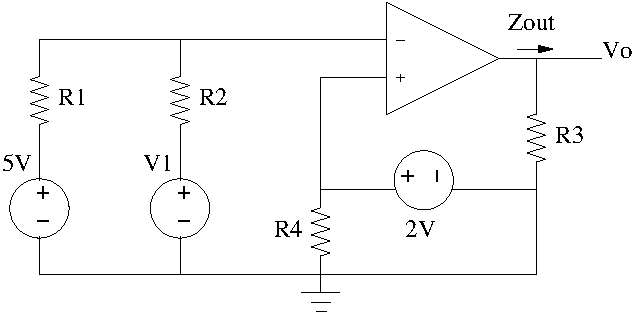
\includegraphics[width=0.6\linewidth]{comparator} &
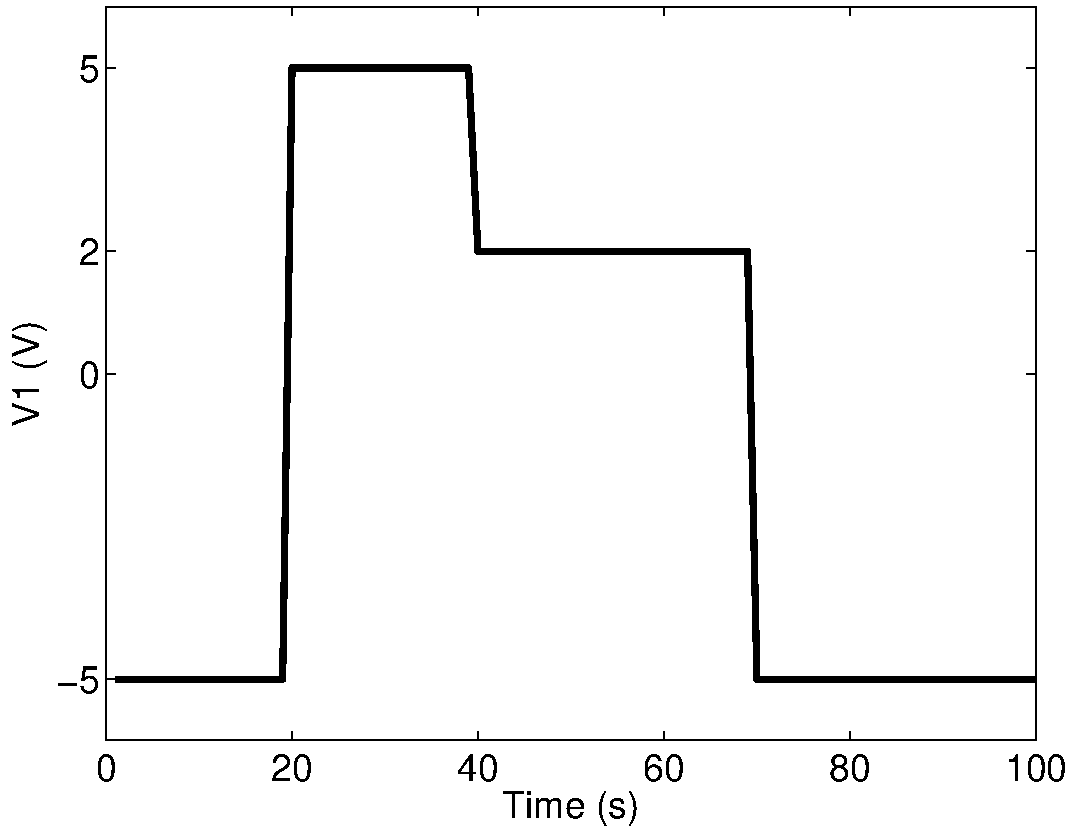
\includegraphics[width=0.4\linewidth]{comparator_v1} \\
\end{tabular}

The op amp in the circuit rails at $\pm$ 12 V.

\begin{enumerate}
    \item Yes, you are getting a multiple choice question; circle your answer.  This circuit has:
    \begin{itemize}
        \item Negative Feedback
        \item Positive Feedback
        \item No Feedback
        \item Both Positive and Negative Feedback
    \end{itemize}
    \item Derive an expression for node voltage of the inverting input of the op amp in terms of $R_1$, $R_2$ and $V_1$.
    \item Assume that $R_1$ = $R_2$ = $R_3$ = $R_4$ and $V_1(t < 0)$ = -5 V.  Given $V_1(t)$ in the plot above, sketch $V_o(t)$.
    \item What is $Z_\textrm{out}$?
    \item How does $V_o(t)$ change if $R_3$ is twice the resistance of the other resistors (i.e., $R_3$ = 2$R_1$ = 2$R_2$ = 2$R_4$)?
\end{enumerate}

\clearpage

{\bf BME154L - Spring 2012 - Exam \#2 Solutions}\hfill Name (Net ID):\underline{\hspace*{3.0in}}



\clearpage
